\section{Introduction}
% Delete the text and write your Introduction here:
%------------------------------------




The problem we aim to solve during this project is the placement of a sensor on a specific target point on a surface using a fixed manipulator arm mounted on the top of an unmanned quadcopter.
A quacopter is an underactuacted helicopter with four rotors. This UAV (Unmanned Aerial Vehicles) is underactuated because arbitrary configurations and trajectory cannot be realized.\\
In the last ten years, research about UAV controls accelerated drastically with many applications in the civilian industry in a variety of areas.\\
Monitoring and sensing tasks are traditionally operated by human but can be complicated (require expert, highly trained technicians), expensive,  and dangerous for the human operator (when the point of interest is hard to reach, the human manipulator may need special training and equipement to reach the point of interest). For example, big structures like bridges need to undergo regular inspections to ensure there are no cracks or other signs of structural fatigue.\\
Using UAVs for such tasks would not only reduce cost of maintance of those structures, but also increase the security of both the human manipulator and the civilians using it. \\
Sensor placement on surfaces using UAVs  is an active field of research and we will propose a solution based on velocity fields.\\

A velocity field is a function taking as input a state, $q$ and returns a 3 dimensional desired velocity vector $(u,v,w)$.\\ It describes a path (a function of position) as opposed to a trajectory (function of position and time).
Diverse ways of placing sensors using UAVs have been explored in the past, including but not limited to: 
\begin{itemize}
    \item Direct Placement: Using a fixed arm manipulator on an UAV, we use the force exerted by the thrust of the UAV to provide enough pressure on the tip of the arm to place the sensor on the target point.
    \item Sensor Launching \cite{farinha2020unmanned}: Using the energy stored in a spring, the UAV ejects the sensor at the desired velocity to reach and attach to the target (Unmanned Aerial Sensor Placement for Cluttered Environments). This strategy is very useful when it is not physically possible for a mounted arm to reach the target however it suffers from small payload capacity.
    \item Drop from flight: We simply drop the sensor above the target point. When target accuracy is not a priority and we are aiming at a non-vertical surface and there is no occlusion above the target,  this sensor placement strategy is the most effective. 
\end{itemize}
\begin{figure}[h!]
    \centering
    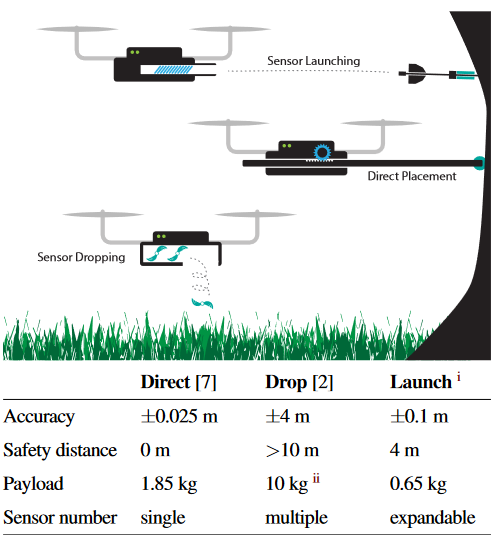
\includegraphics[width=0.48\textwidth]{Images/threeway.png}
    \caption{Different types of sensor placement from \cite{farinha2020unmanned}}
    \label{fig:threeway}
\end{figure}
The characteristics of each one of mentioned methods are shown in \ref{fig:threeway}.
We decided to go through with the Direct Placement strategy because despite its simplicity, it provides good accuracy and is able to place a large variety of payloads. 
The solution we will propose can be divided in 3 parts: The first is environment mapping where we perform surface and obstacle recognition using live depth sensor feed. The second part is designing a potential based velocity field to perform path-planning by guiding the UAV from the start point to the target point. The third and last part is designing a velocity field around the target point to apply the desired force amplitude. In this part, we will use the passive velocity field controller (PVFC) to optimize our energy consumption.
